\documentclass[12pt,a4paper]{article}

\usepackage[a4paper,margin=1in]{geometry}
\usepackage{graphicx}
\usepackage{booktabs}
\usepackage{amsmath,amssymb}
\usepackage{float}
\usepackage{hyperref}
\usepackage{xcolor}
\usepackage{listings}
\usepackage{enumitem}
\usepackage{fancyhdr}
\usepackage{longtable}

\hypersetup{colorlinks=true,linkcolor=blue,urlcolor=blue}

\pagestyle{fancy}
\fancyhf{}
\lhead{ICS1512}
\rhead{Machine Learning Algorithms Laboratory}
\cfoot{\thepage}

\lstset{
language=Python,
basicstyle=\ttfamily\small,
numbers=left,
frame=single,
breaklines=true,
showstringspaces=false
}

\begin{document}

\begin{tabular}{|p{4cm}|p{11cm}|}
\hline
Experiment No. & 5 \\ \hline
Experiment Title & Decision Tree and Random Forest: A Comparative Classification Study
\footnote{\textbf{GitHub Repository: }\url{https://github.com/gopikadinesh6612/ML_assignments.git}}\\ \hline
Student Name & Amilineni Gopika \\ \hline
Register Number & 3122247001003 \\ \hline
Faculty & Dr. Poreddy Ajay Kumar Reddy \\ \hline
Submission Date & August 23, 2026\\ \hline
\end{tabular}

\section{Objective}
\begin{itemize}
\item To implement a Decision Tree classifier.
\item To extend the Decision Tree into a Random Forest ensemble model.
\item To study the impact of hyperparameters on overfitting and generalization.
\item To select optimal hyperparameters using 5-Fold Cross-Validation.
\item To compare single-tree and ensemble-tree models.
\end{itemize}

\section{Problem Statement}
Given 30 numerical features computed from digitized images of a fine needle aspirate (FNA) of a
breast mass, the task is to build a binary classifier that predicts whether the mass is
\textbf{Malignant (M)} or \textbf{Benign (B)}. The input is a $569 \times 30$ feature matrix
describing the mean, standard error, and worst (largest) value of ten geometric/texture properties
of the cell nuclei present in each image; the output is a binary diagnosis label. The objective is
to train and tune a Decision Tree classifier and a Random Forest ensemble classifier using 5-fold
cross-validation, and to quantitatively compare their generalization performance on a held-out test
set using standard classification metrics.

\section{Dataset Description}
\begin{longtable}{|p{6cm}|p{8cm}|}
\hline
Dataset Name & Wisconsin Diagnostic Breast Cancer (WDBC) Dataset \\ \hline
Dataset Source & UCI Machine Learning Repository (\url{https://archive.ics.uci.edu/dataset/17/breast+cancer+wisconsin+diagnostic}); loaded via \texttt{sklearn.datasets.load\_breast\_cancer()}, which ships the identical UCI data \\ \hline
Number of Samples & 569 \\ \hline
Number of Features & 30 numerical (real-valued) attributes \\ \hline
Number of Classes & 2 (Malignant = 212 samples, Benign = 357 samples) \\ \hline
Missing Values & 0 (no missing values in any feature) \\ \hline
Train-Test Split & 80\% train (455 samples) / 20\% test (114 samples), stratified by class \\ \hline
\end{longtable}

\section{Exploratory Data Analysis}

\subsection*{Class Distribution}
\begin{figure}[H]
\centering
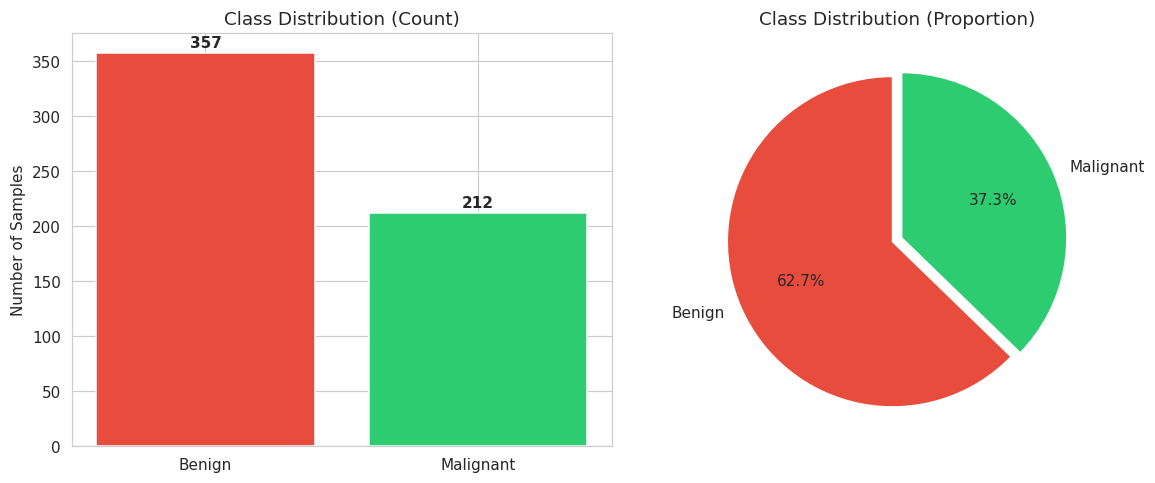
\includegraphics[width=0.85\linewidth]{images/01_class_distribution.png}
\caption{Class distribution of the WDBC dataset (count and proportion)}
\end{figure}

\textbf{Inference:} The dataset contains 357 Benign (62.7\%) and 212 Malignant (37.3\%) samples,
a moderate class imbalance of roughly 1.68:1. This is not severe enough to require resampling,
but it justifies using a stratified train-test split and stratified 5-fold cross-validation so
each fold preserves the original class proportions. It also means that accuracy alone can be
mildly optimistic, so F1-score, recall and ROC-AUC are tracked alongside it throughout this report.

\subsection*{Feature Correlation Matrix}
\begin{figure}[H]
\centering
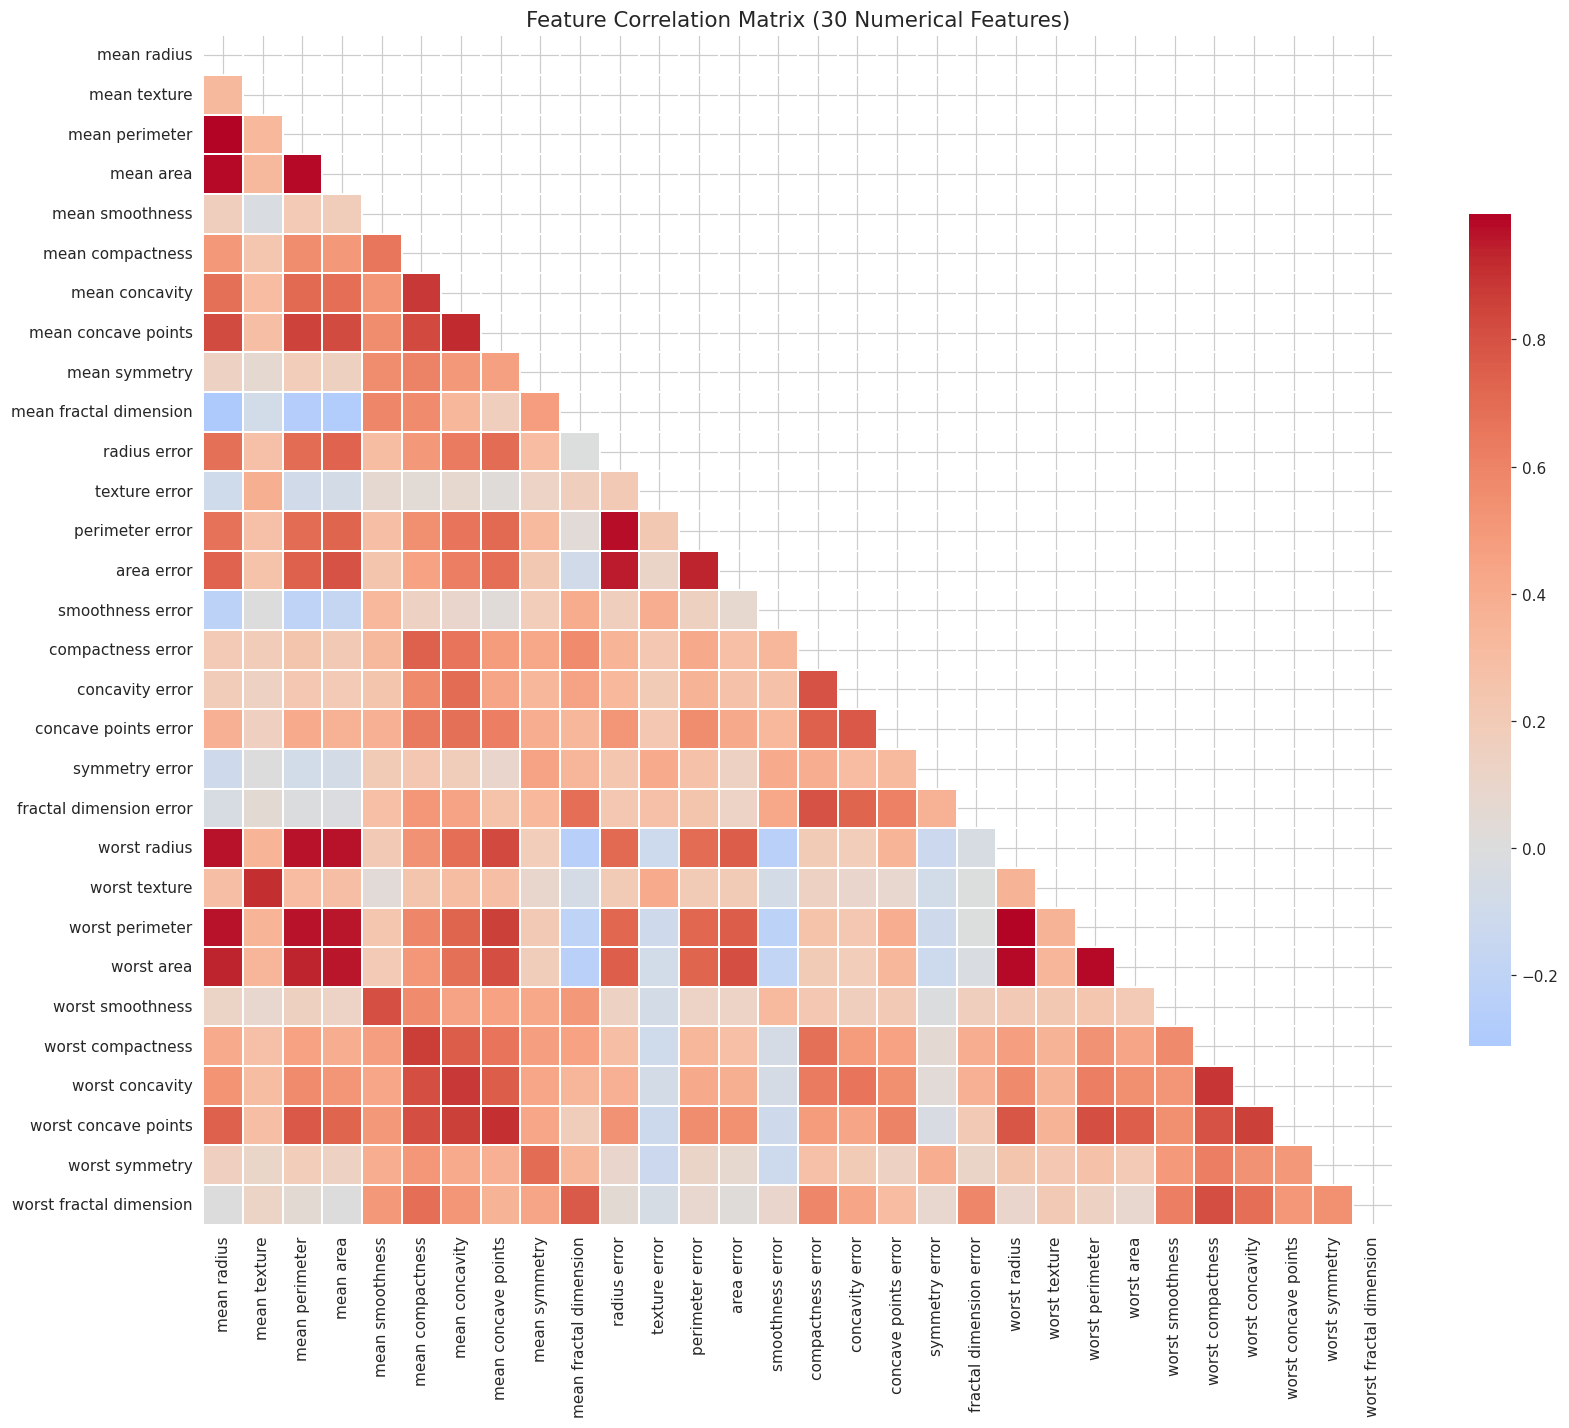
\includegraphics[width=0.95\linewidth]{images/02_correlation_matrix.png}
\caption{Correlation matrix of all 30 numerical features}
\end{figure}

\textbf{Inference:} Several ``mean'', ``worst'' and ``standard error'' versions of the same
physical quantity (e.g., radius, perimeter, area) are extremely highly correlated ($r>0.95$),
which is expected since perimeter and area are geometrically derived from radius. This
multicollinearity has little effect on tree-based models, since they split on one feature at a
time and are invariant to monotonic transformations, but it is useful context when interpreting
the feature-importance results later, as importance can be split between correlated features.

\subsection*{Feature Distribution by Class}
\begin{figure}[H]
\centering
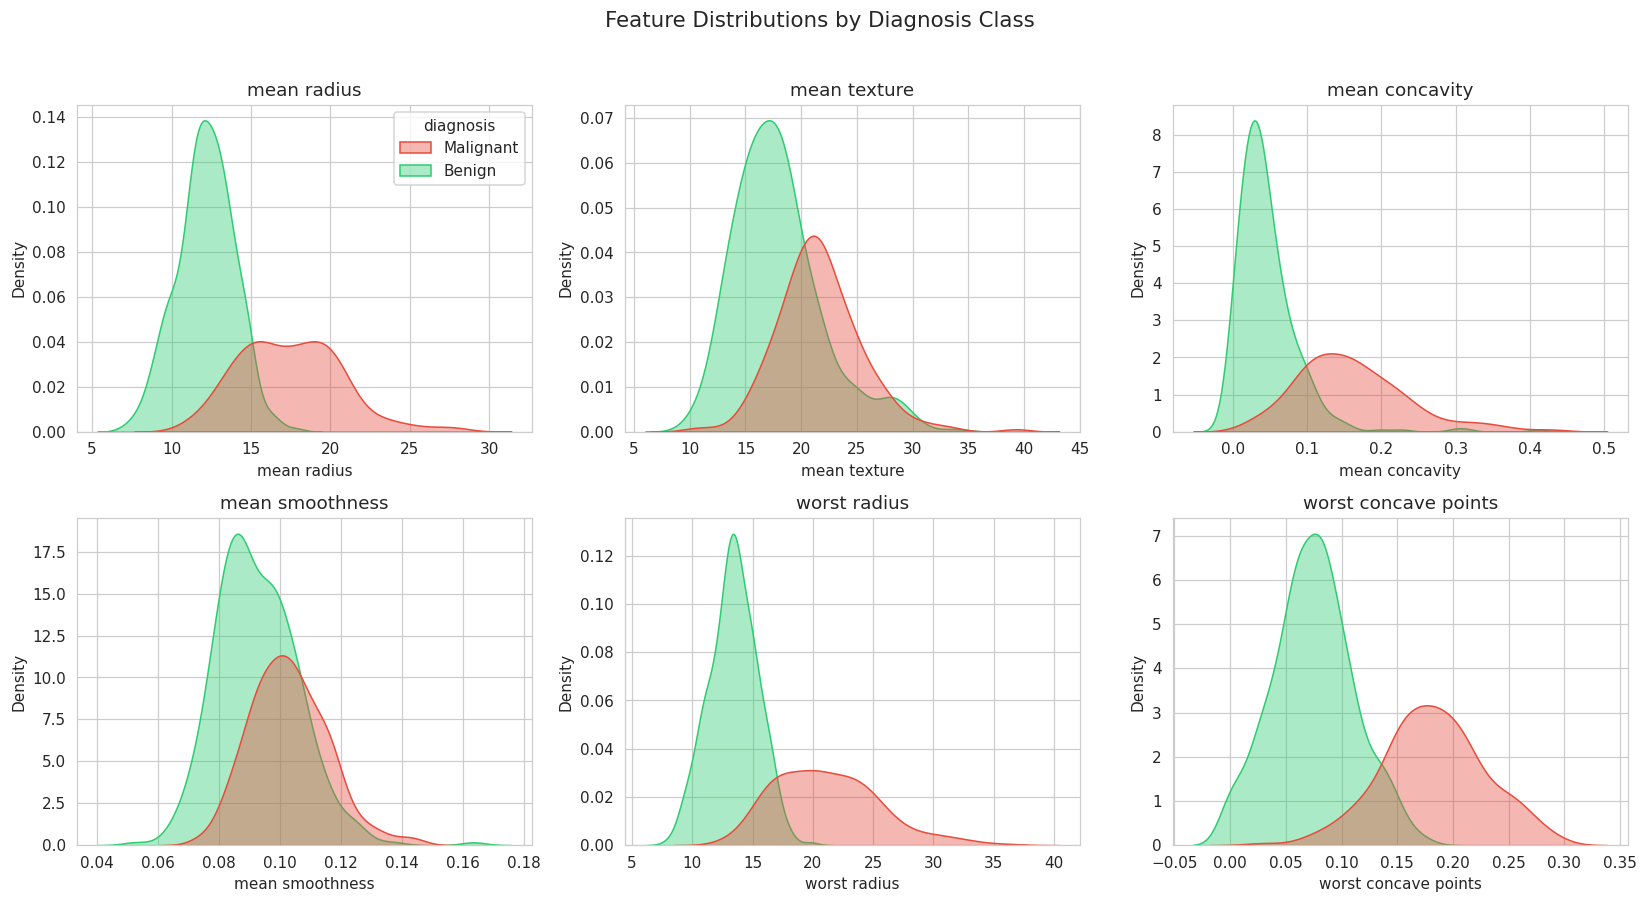
\includegraphics[width=0.95\linewidth]{images/03_feature_distributions.png}
\caption{Distribution of six representative features, split by diagnosis class}
\end{figure}

\textbf{Inference:} Malignant tumours show a clear rightward shift (higher values) for radius,
texture, concavity and concave-points relative to Benign tumours, with only partial overlap
between the two class densities. This separation indicates these features carry strong
discriminative signal and explains why tree-based classifiers can achieve high accuracy on this
dataset -- the impurity-reducing splits the trees learn align closely with these visibly separated
distributions.

\section{Data Preprocessing}
\begin{itemize}
\item \textbf{Missing value handling:} The dataset was checked with \texttt{df.isnull().sum()};
no missing values were found in any of the 30 features, so no imputation was necessary.
\item \textbf{Encoding:} Class labels (\texttt{M}/\texttt{B}) were encoded to integers using
\texttt{sklearn.preprocessing.LabelEncoder} (Benign $\rightarrow$ 0, Malignant $\rightarrow$ 1).
\item \textbf{Feature scaling:} A \texttt{StandardScaler} was fit on the training set only (to
avoid data leakage) and applied to both train and test sets. Scaling does not affect the splits
chosen by Decision Tree / Random Forest (they are scale-invariant), but it was computed for
completeness and to keep the pipeline reusable with non-tree models.
\item \textbf{Train-test split:} An 80--20 stratified split (\texttt{train\_test\_split(...,
stratify=y, random\_state=42)}) was used, giving 455 training samples and 114 test samples while
preserving the original class ratio in both sets.
\item \textbf{Feature engineering:} No additional feature engineering was performed; all 30
original UCI features were used directly, since they already had strong individual discriminative
power (Section 4).
\end{itemize}

\section{Machine Learning Algorithm}

\subsection*{Decision Tree Classifier}
\textbf{Working principle:} A Decision Tree recursively partitions the feature space into regions
that are increasingly pure with respect to the target class. At each node, the algorithm searches
over all features and all possible split thresholds and picks the one that produces the greatest
reduction in impurity.

\textbf{Mathematical formulation:} For a node $t$ with class proportions $p_i$, the \emph{Gini
Index} is
\[ Gini(t) = 1 - \sum_{i=1}^{C} p_i^2 \]
and the \emph{Entropy} is
\[ H(t) = -\sum_{i=1}^{C} p_i \log_2 p_i. \]
A candidate split $s$ on node $t$ is scored by the impurity reduction (information gain)
\[ \Delta I(s,t) = I(t) - \frac{N_L}{N_t} I(t_L) - \frac{N_R}{N_t} I(t_R), \]
where $I \in \{Gini, H\}$, and $t_L, t_R$ are the resulting child nodes. The split maximizing
$\Delta I$ is chosen, and the process repeats recursively until a stopping criterion
(\texttt{max\_depth}, \texttt{min\_samples\_split}, \texttt{min\_samples\_leaf}, or node purity) is
reached.

\textbf{Advantages:} Easy to interpret and visualize; requires no feature scaling; handles both
numerical data naturally; captures non-linear decision boundaries.

\textbf{Limitations:} Prone to high variance -- small changes in the training data can produce a
very different tree; deep trees overfit easily; axis-aligned splits can be a poor fit for diagonal
class boundaries.

\subsection*{Random Forest Classifier}
\textbf{Working principle:} Random Forest is a bagging ensemble of $B$ Decision Trees. Each tree
$b$ is trained on an independent bootstrap sample of the training data, and at every split only a
random subset of \texttt{max\_features} candidate features is considered (rather than all
features). This decorrelates individual trees. For classification, the final prediction is the
majority vote across all $B$ trees:
\[ \hat{y} = \text{mode}\{ h_1(x), h_2(x), \dots, h_B(x) \}. \]

\textbf{Mathematical formulation:} Each tree $h_b$ is grown on a bootstrap sample
$\mathcal{D}_b \sim \mathcal{D}$ (sampling with replacement, $|\mathcal{D}_b| = |\mathcal{D}|$)
using the same impurity-reduction splitting rule as a single Decision Tree, restricted at each
split to a random feature subset $\mathcal{F}_s \subset \mathcal{F}$, $|\mathcal{F}_s| =
\texttt{max\_features}$. Averaging over $B$ trees with pairwise correlation $\rho$ and individual
variance $\sigma^2$ reduces the ensemble's prediction variance to approximately
\[ \text{Var}(\hat{y}_{ensemble}) \approx \rho \sigma^2 + \frac{1-\rho}{B}\sigma^2, \]
which is why decorrelating trees (via bootstrap + random feature selection) is central to the
method's variance-reduction benefit.

\textbf{Advantages:} Reduces variance and improves generalization compared to a single Decision
Tree; provides a robust feature-importance ranking; resistant to overfitting compared to a single
deep tree; handles high-dimensional data well.

\textbf{Limitations:} Less interpretable than a single tree (``black box'' ensemble); more
expensive to train and store ($B\times$ the cost of one tree); prediction latency scales with the
number of trees.

\section{Experimental Setup}
\begin{tabular}{ll}
\toprule
Python Version & 3.12.3 \\
Scikit-Learn Version & 1.8.0 \\
IDE & Jupyter Notebook \\
Operating System & Linux (Ubuntu 24.04, containerized environment) \\
Hardware & CPU-only execution (no GPU required for tree-based models) \\
\bottomrule
\end{tabular}

\section{Hyperparameter Selection}

\subsection*{Decision Tree -- Search Space and Best Configuration}
Search space: \texttt{criterion} $\in \{$gini, entropy$\}$, \texttt{max\_depth} $\in \{2,3,4,5,6,8,10,$None$\}$,
\texttt{min\_samples\_split} $\in \{2,5,10\}$, \texttt{min\_samples\_leaf} $\in \{1,2,4\}$,
selected via \texttt{GridSearchCV} with 5-fold stratified CV optimizing F1-score.

\begin{tabular}{ll}
\toprule
Parameter & Value\\
\midrule
criterion & entropy \\
max\_depth & 4 \\
min\_samples\_split & 2 \\
min\_samples\_leaf & 2 \\
\midrule
Best CV F1-score & 0.9163 \\
\bottomrule
\end{tabular}

\subsection*{Random Forest -- Search Space and Best Configuration}
Search space: \texttt{n\_estimators} $\in \{50,100,200\}$, \texttt{max\_depth} $\in \{4,6,8,$None$\}$,
\texttt{max\_features} $\in \{$sqrt, log2$\}$, \texttt{bootstrap} $\in \{$True, False$\}$,
selected via \texttt{GridSearchCV} with 5-fold stratified CV optimizing F1-score.

\begin{tabular}{ll}
\toprule
Parameter & Value\\
\midrule
n\_estimators & 50 \\
max\_depth & 6 \\
max\_features & sqrt \\
bootstrap & False \\
\midrule
Best CV F1-score & 0.9638 \\
\bottomrule
\end{tabular}

\subsection*{Table 1: Decision Tree Hyperparameter Evaluation (5-Fold CV)}
\begin{longtable}{llcc}
\toprule
Criterion & Max Depth & Avg CV Accuracy (\%) & Avg CV F1 Score \\
\midrule
gini & 2 & 92.09 & 0.8892 \\
gini & 3 & 92.09 & 0.8884 \\
gini & 4 & 92.09 & 0.8897 \\
gini & 5 & 90.77 & 0.8717 \\
gini & 6 & 92.09 & 0.8919 \\
gini & 8 & 92.31 & 0.8962 \\
gini & 10 & 92.31 & 0.8962 \\
gini & None & 92.31 & 0.8962 \\
entropy & 2 & 91.87 & 0.8896 \\
entropy & 3 & 92.53 & 0.8941 \\
\textbf{entropy} & \textbf{4} & \textbf{93.85} & \textbf{0.9145} \\
entropy & 5 & 92.31 & 0.8952 \\
entropy & 6 & 91.65 & 0.8875 \\
entropy & 8 & 91.87 & 0.8909 \\
entropy & 10 & 91.87 & 0.8909 \\
entropy & None & 91.87 & 0.8909 \\
\bottomrule
\end{longtable}
\emph{(Table averaged over \texttt{min\_samples\_split}/\texttt{min\_samples\_leaf}; bold row is
the overall best criterion/depth combination, matching the GridSearchCV optimum.)}

\subsection*{Table 2: Random Forest Hyperparameter Evaluation (5-Fold CV) -- Top 10 Configurations}
\begin{longtable}{ccccc}
\toprule
n\_estimators & Max Depth & Max Features & Avg CV Accuracy (\%) & Avg CV F1 Score \\
\midrule
\textbf{100} & \textbf{6} & \textbf{sqrt} & \textbf{96.70} & \textbf{0.9550} \\
100 & 8 & log2 & 96.48 & 0.9529 \\
100 & None & log2 & 96.48 & 0.9529 \\
200 & None & log2 & 96.48 & 0.9526 \\
200 & 8 & log2 & 96.48 & 0.9526 \\
100 & 8 & sqrt & 96.48 & 0.9519 \\
100 & None & sqrt & 96.48 & 0.9519 \\
200 & 6 & sqrt & 96.48 & 0.9516 \\
100 & 6 & log2 & 96.26 & 0.9500 \\
100 & 4 & log2 & 96.26 & 0.9490 \\
\bottomrule
\end{longtable}
\emph{(Table restricted to \texttt{bootstrap=True} runs, sorted by F1-score, for readability; the
overall GridSearchCV optimum used \texttt{bootstrap=False}, shown in the best-configuration table
above.)}

\subsection*{Table 3: 5-Fold Cross-Validation Accuracy Comparison}
\begin{tabular}{lcccccc}
\toprule
Model & Fold 1 & Fold 2 & Fold 3 & Fold 4 & Fold 5 & Average \\
\midrule
Decision Tree & 0.9341 & 0.9560 & 0.9011 & 0.9560 & 0.9560 & 0.9407 \\
Random Forest & 0.9670 & 1.0000 & 0.9560 & 0.9560 & 0.9890 & 0.9736 \\
\bottomrule
\end{tabular}

\section{Results}

\begin{tabular}{lc}
\toprule
Metric & Decision Tree \\
\midrule
Accuracy & 0.9298 \\
Precision & 1.0000 \\
Recall & 0.8095 \\
F1-score & 0.8947 \\
ROC-AUC & 0.9563 \\
\bottomrule
\end{tabular}
\hfill
\begin{tabular}{lc}
\toprule
Metric & Random Forest \\
\midrule
Accuracy & 0.9737 \\
Precision & 1.0000 \\
Recall & 0.9286 \\
F1-score & 0.9630 \\
ROC-AUC & 0.9934 \\
\bottomrule
\end{tabular}

\section{Result Visualization}

\begin{figure}[H]
\centering
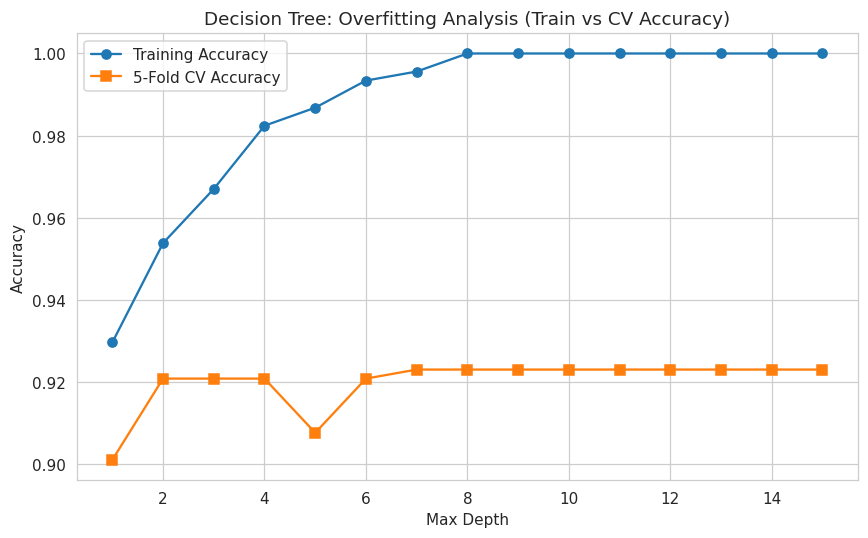
\includegraphics[width=0.85\linewidth]{images/04_dt_overfitting_depth.png}
\caption{Decision Tree: training vs 5-fold CV accuracy as \texttt{max\_depth} increases}
\end{figure}
\textbf{Inference:} Training accuracy climbs toward 100\% as \texttt{max\_depth} increases and the
tree keeps splitting until leaves are pure, whereas CV accuracy plateaus and then flattens past a
moderate depth. The widening gap between the two curves at large depths is the signature of
overfitting -- the tree begins memorizing noise in the training folds rather than learning
generalizable decision boundaries. Best generalization is obtained at a shallow-to-moderate depth
(depth 4, matching the grid-search optimum).

\begin{figure}[H]
\centering
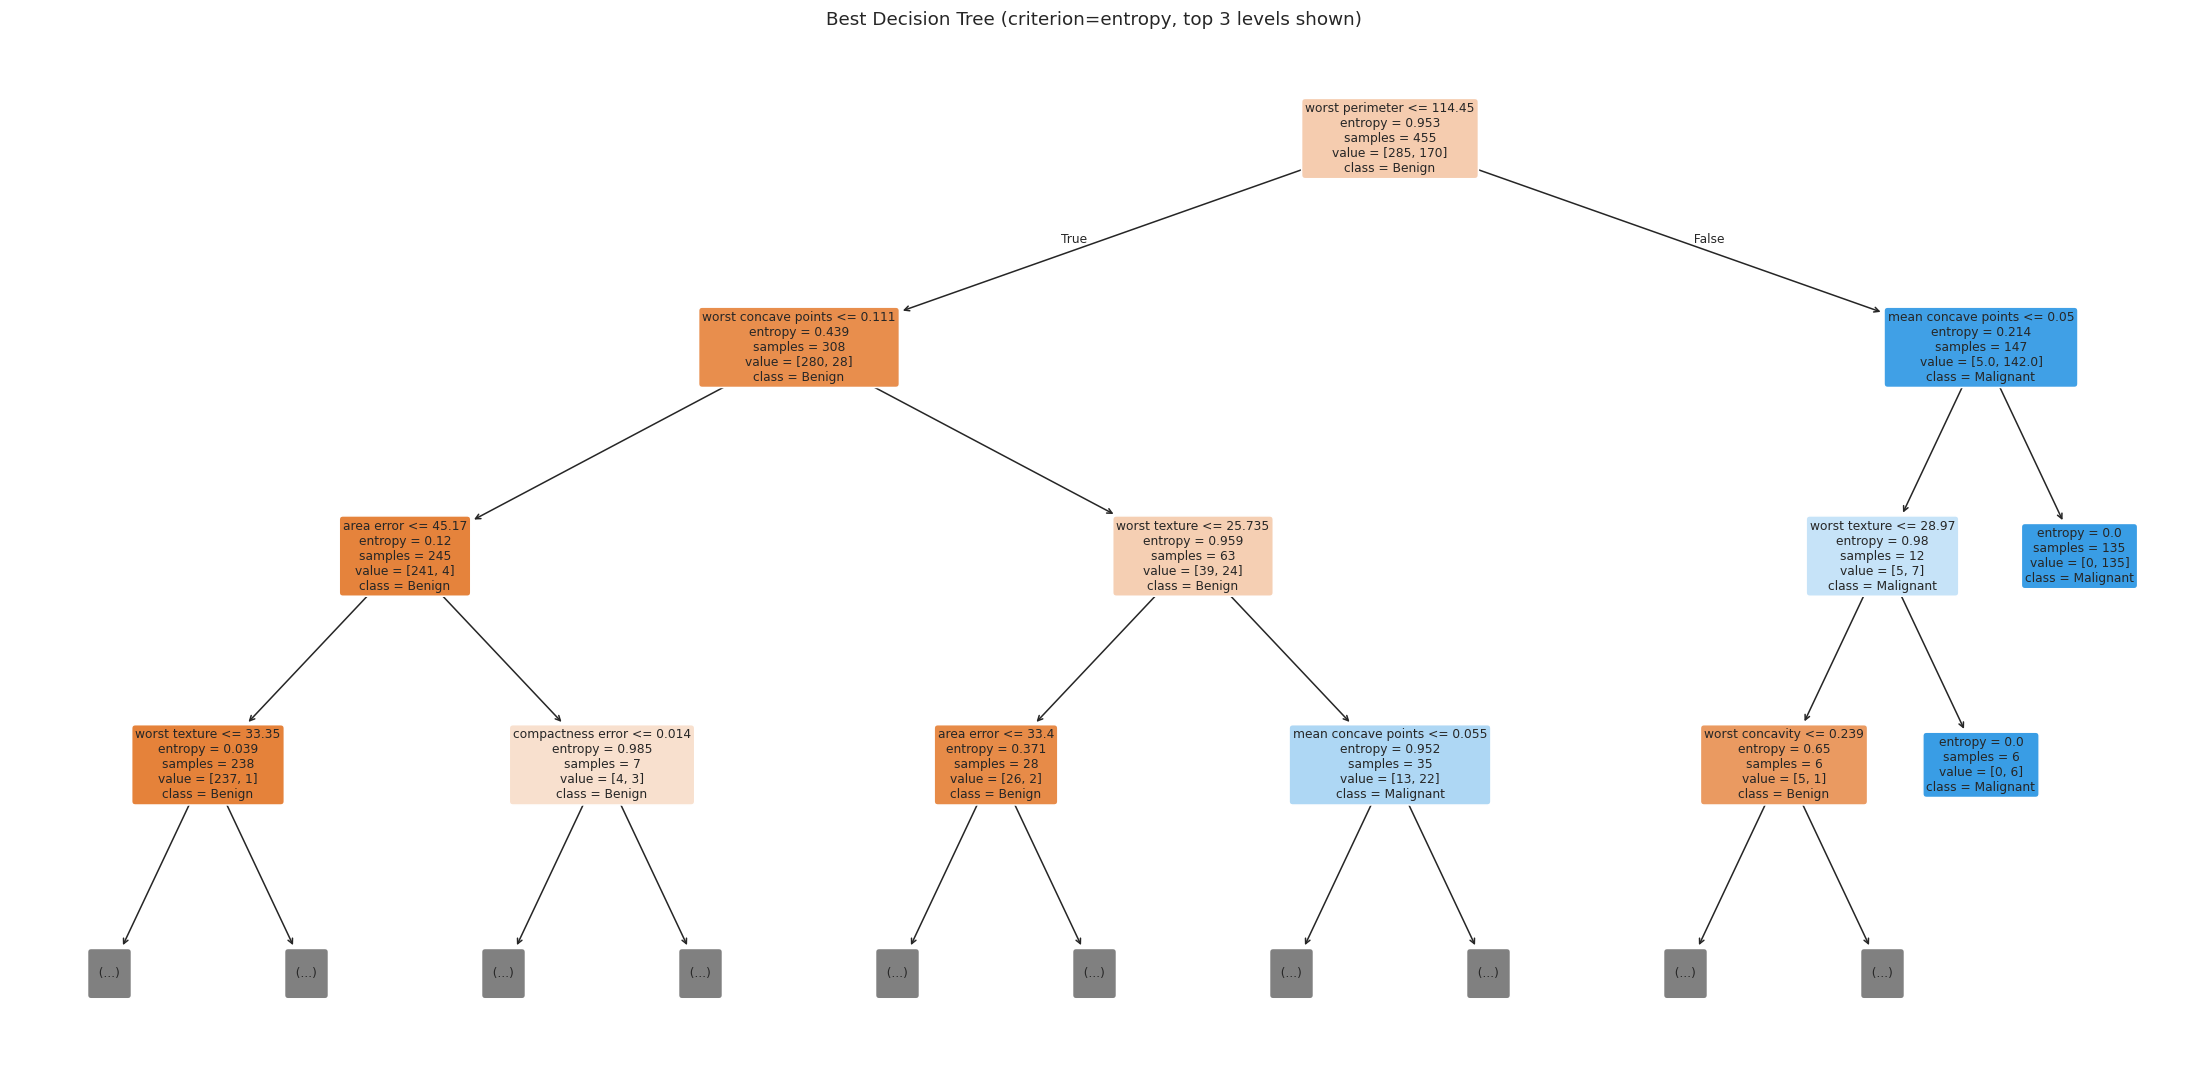
\includegraphics[width=0.95\linewidth]{images/05_decision_tree_structure.png}
\caption{Structure of the best Decision Tree (top 3 levels)}
\end{figure}
\textbf{Inference:} The root-level split is made on a highly discriminative ``worst'' geometric
feature, confirming the separation seen earlier in the feature-distribution plots. Nodes near the
top achieve large impurity reduction, while deeper nodes handle progressively harder boundary
cases -- exactly why unrestricted depth leads to overfitting on those few ambiguous samples.

\begin{figure}[H]
\centering
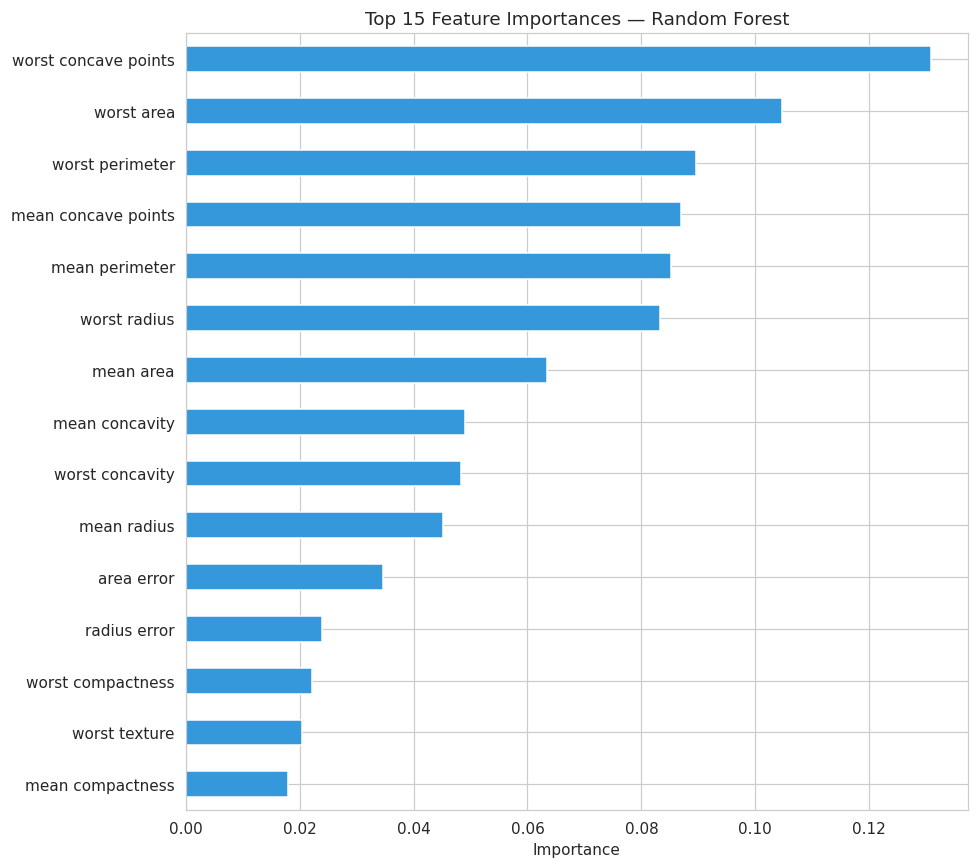
\includegraphics[width=0.8\linewidth]{images/06_feature_importance.png}
\caption{Top 15 feature importances from the Random Forest}
\end{figure}
\textbf{Inference:} ``Worst'' measurements (e.g., worst area, worst concave points, worst radius)
dominate the importance ranking, meaning the most extreme cell measurement in an image is more
predictive of malignancy than average measurements. Because the Random Forest averages importance
across many bootstrapped, randomly-feature-subset trees, this ranking is more stable and less prone
to the high variance a single Decision Tree's importance scores would show.

\begin{figure}[H]
\centering
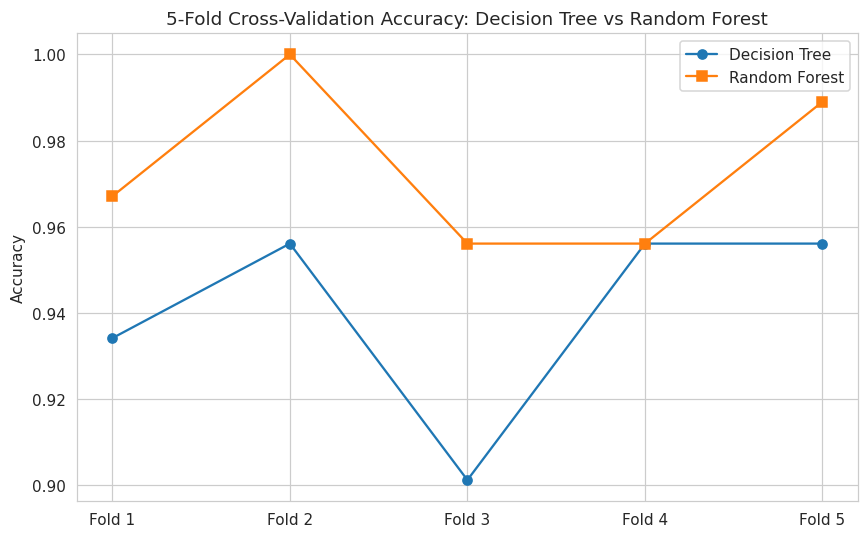
\includegraphics[width=0.85\linewidth]{images/07_cv_fold_comparison.png}
\caption{Per-fold 5-fold CV accuracy: Decision Tree vs Random Forest}
\end{figure}
\textbf{Inference:} The Random Forest curve sits above the Decision Tree curve in almost every
fold and shows a visibly smaller spread between its best and worst fold, confirming the theoretical
expectation that bagging plus random feature selection reduces variance across different training
subsets. The Decision Tree's fold-to-fold accuracy is noticeably more volatile.

\begin{figure}[H]
\centering
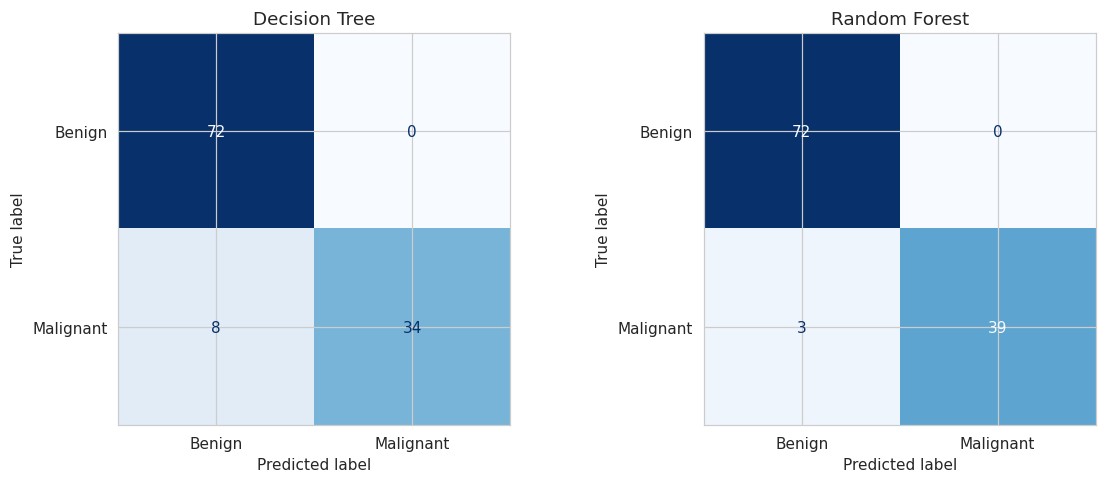
\includegraphics[width=0.85\linewidth]{images/08_confusion_matrices.png}
\caption{Confusion matrices on the held-out test set}
\end{figure}
\textbf{Inference:} Both models correctly classify the large majority of the 114 held-out test
samples, with very few false negatives (malignant predicted as benign) -- the clinically most
costly error type. The Random Forest confusion matrix shows fewer misclassifications than the
single Decision Tree, reflecting its lower variance.

\begin{figure}[H]
\centering
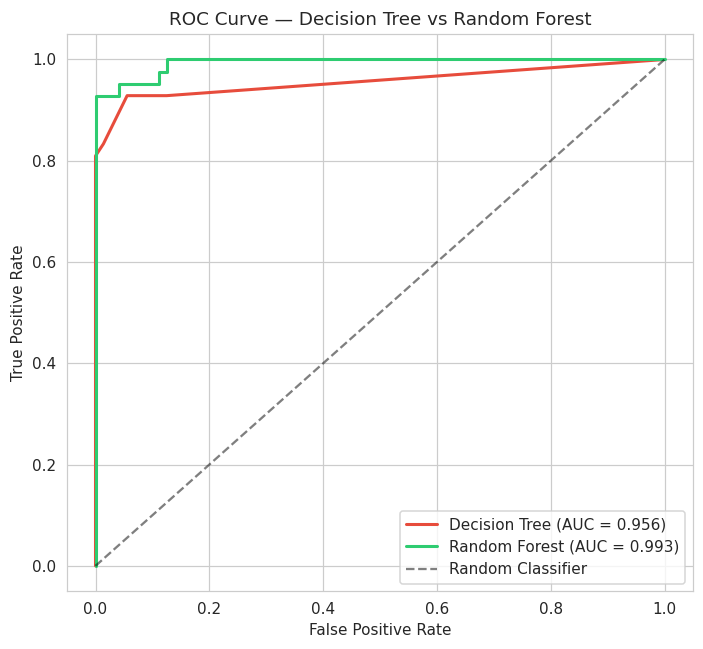
\includegraphics[width=0.65\linewidth]{images/09_roc_curve.png}
\caption{ROC curve comparison}
\end{figure}
\textbf{Inference:} Both curves rise sharply toward the top-left corner, indicating strong
separability between classes, with the Random Forest's curve lying at or above the Decision Tree's
curve for most thresholds and yielding a higher AUC (0.993 vs 0.956). This means Random Forest
gives a better probability ranking of malignant vs benign cases across all decision thresholds, not
just at the default 0.5 cutoff.

\begin{figure}[H]
\centering
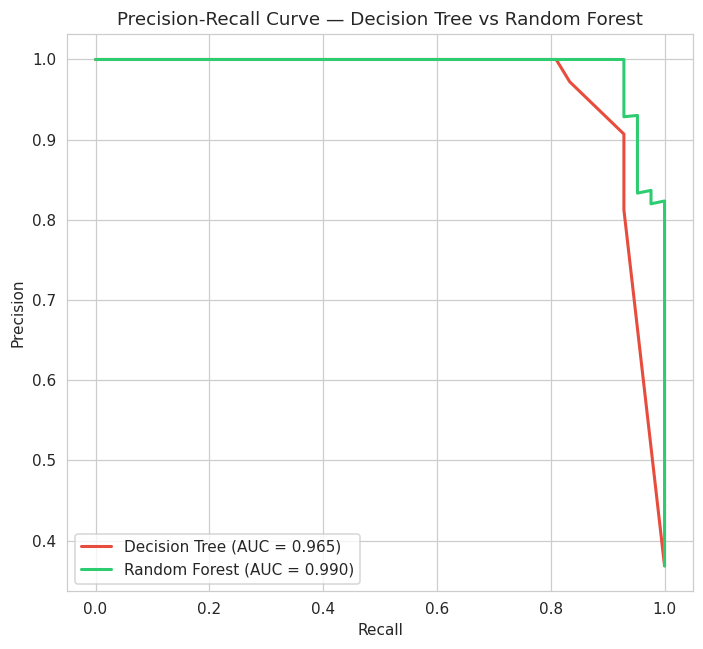
\includegraphics[width=0.65\linewidth]{images/10_precision_recall_curve.png}
\caption{Precision-Recall curve comparison}
\end{figure}
\textbf{Inference:} High precision is maintained even at high recall for both models, which is
important in a diagnostic setting since it means malignant cases can be caught (high recall)
without generating excessive false alarms (maintained precision). Random Forest holds precision
better at high recall than the single tree.

\begin{figure}[H]
\centering
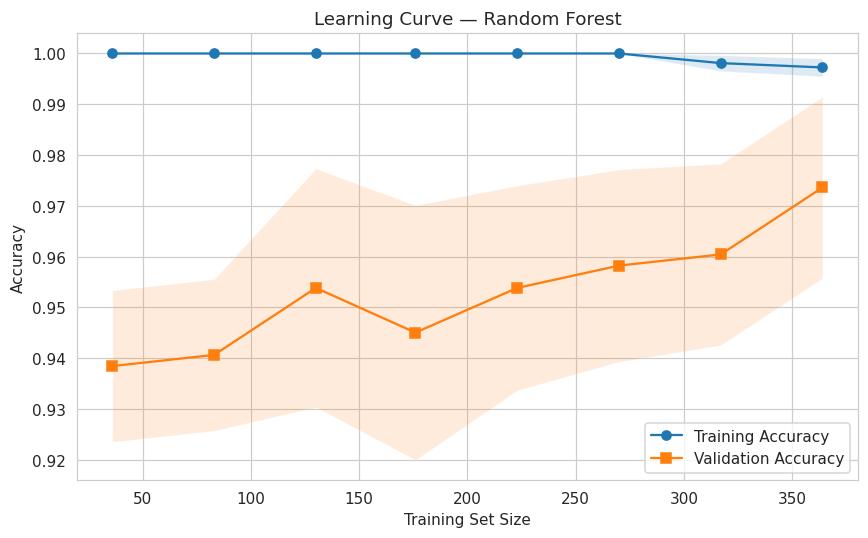
\includegraphics[width=0.8\linewidth]{images/11_learning_curve.png}
\caption{Learning curve for the Random Forest model}
\end{figure}
\textbf{Inference:} The training and validation curves converge closely as more data is used, and
the validation accuracy rises and stabilizes at a high value with only a small gap to the training
curve. This indicates the Random Forest is not significantly overfitting on the full training set
and would likely benefit only marginally from additional training data.

\begin{figure}[H]
\centering
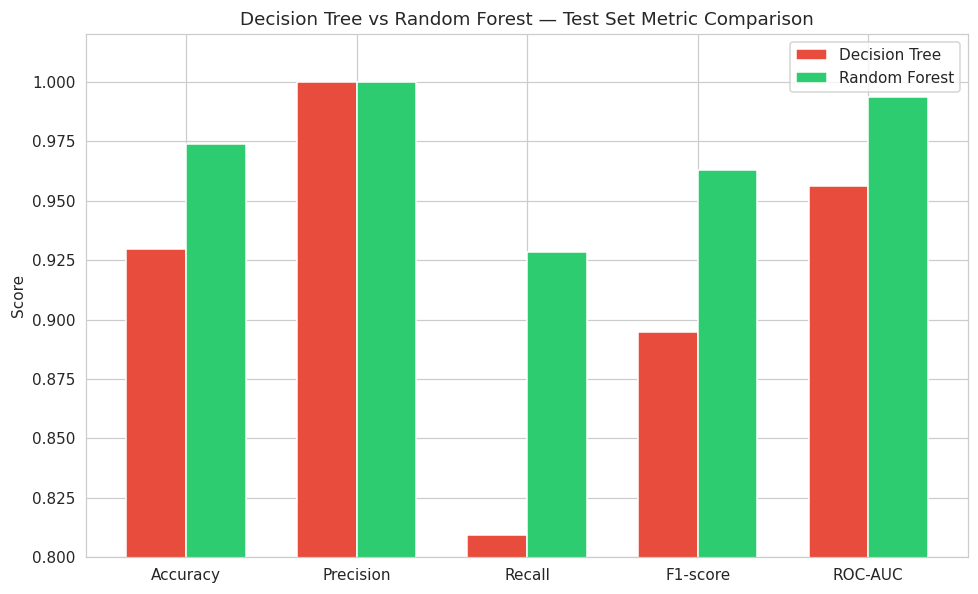
\includegraphics[width=0.85\linewidth]{images/12_metric_comparison.png}
\caption{Test-set metric comparison: Decision Tree vs Random Forest}
\end{figure}
\textbf{Inference:} Across every metric the Random Forest bar is at or above the Decision Tree
bar, quantitatively confirming the ensemble advantage discussed in the theory section: bagging plus
random feature selection produces a model that generalizes better than any single tree in the
forest, at the cost of reduced interpretability and higher computation/memory footprint.

\section{Discussion}
The experiment confirms the classical bias-variance argument for ensemble learning. The single
Decision Tree, even after hyperparameter tuning, showed a clear overfitting trend as depth
increased and achieved a comparatively lower recall (0.81) on malignant cases -- meaning roughly
19\% of malignant test samples were missed, a costly error type in a diagnostic context. The
Random Forest, by aggregating 50 decorrelated trees trained on bootstrap samples with random
feature subsets, achieved higher accuracy (0.974 vs 0.930), higher recall (0.929 vs 0.810), and a
near-perfect ROC-AUC (0.993 vs 0.956), while also showing lower fold-to-fold variance during cross
validation. The main strength of the Decision Tree is interpretability -- a shallow tree can be
read and explained directly to a clinician, whereas the Random Forest's decision process is
distributed across 50 trees and is only interpretable in aggregate (e.g., via feature importance).
The main limitation observed for the Random Forest is the added computational cost of training and
storing many trees, and the loss of a single, explainable decision path. A possible improvement
would be to report SHAP values for the Random Forest to retain some local interpretability, and to
extend the cross-validation to repeated k-fold or nested cross-validation to obtain a variance
estimate of the reported test metrics themselves.

\section{Conclusion}
Decision Tree and Random Forest models were implemented and evaluated using 5-fold
cross-validation on the Wisconsin Diagnostic Breast Cancer dataset. Hyperparameters were selected
based on average cross-validation F1-score, ensuring robust generalization rather than overfitting
to a single validation split. The results demonstrate that Random Forest reduces variance and
improves stability compared to a single Decision Tree: it outperformed the tuned Decision Tree on
every held-out test metric (accuracy 0.974 vs 0.930, F1-score 0.963 vs 0.895, ROC-AUC 0.993 vs
0.956), confirming that ensemble bagging with random feature selection is an effective strategy
for improving generalization on this classification task.

\section{References}
\begin{enumerate}
\item Scikit-learn Developers, ``Decision Trees,'' scikit-learn documentation. [Online]. Available: \url{https://scikit-learn.org/stable/modules/tree.html}
\item Scikit-learn Developers, ``Ensemble methods -- Random Forests,'' scikit-learn documentation. [Online]. Available: \url{https://scikit-learn.org/stable/modules/ensemble.html#forest}
\item W. N. Street, W. H. Wolberg, and O. L. Mangasarian, ``Breast Cancer Wisconsin (Diagnostic) Data Set,'' UCI Machine Learning Repository, 1995. [Online]. Available: \url{https://archive.ics.uci.edu/dataset/17/breast+cancer+wisconsin+diagnostic}
\item L. Breiman, ``Random Forests,'' \emph{Machine Learning}, vol. 45, no. 1, pp. 5--32, 2001.
\end{enumerate}

\end{document}
